\chapter{Classification}
Pour effectuer une classification, il faut préciser le critère de classification. Le critère le plus utilisé est celui de la distance entre entités communicantes.
	\begin{enumerate}
		\item Architectures des calculateurs / Architecture de communication
		\item LAN\footnote{Local Area Network} ou RLE\footnote{Réseau Local d'Entreprise}
		\item WAN\footnote{Wide Area Network} ou RLD\footnote{Réseau Longue Distance}
		\item DAN\footnote{Departmental Area Network}, MAN\footnote{Metropolitain Area Network}\ldots
	\end{enumerate}
	\begin{tabular}{| c c c |}
		\hline
		Distance & & Exemple\\
		1m & Square meter & PAN\\
		\hline
		10m & Room & LAN\\
		\hline
		100m & Building & LAN\\
		\hline
		1km & Campus & LAN, DAN\\
		\hline
		100 km & City & WAN\\
		\hline
		1000km & Continent & WAN\\
		\hline
		10 000km & Planet & WAN, The Internet\\
		\hline
	\end{tabular}
Prenons un ordinateur et considérons son architecture. Nous remarquons que des données sont acheminées entre entités sur des bus de communication. Il existe même une coopération entre processeur de traitement et co-processeurs (mathématique, graphique\ldots). Dans certaines architectures différents processeurs de traitement coopèrent selon des schémas bien établis (pipeline, SIMD, MIMD\ldots). Bien que certains problèmes rencontrés dans l'architecture d'un ordinateur se rapprochent de ceux d'un réseau informatique, la discipline `` Architecture des calculateurs '' est à distinguer de la discipline `` Architecture de Communication ''. En effet, la première s'intéresse essentiellement à ce qui se passe à l'intérieur d'un ordinateur, tandis que la seconde s'intéresse à la communication dans sa globalité. C'est pourquoi nous commençons à parler de Réseau lorsque des systèmes autonomes (ex. le calculateur) sont reliés entre eux.

Si la distance est inférieure à 1 m, nous parlons de PAN (Personal Area Network) pour intrconnecter les équipements personnels tels que GSM, portables, organiseurs\ldots

Si l'environnement est local, nous parlons de RLE (Réseau Local d'Entreprise) ou LAN (Local Area Network).

Si la distance est plus grande, nous parlons de RLD (Réseau Longue Distance) ou WAN (Wide Area Network).

En réalité, cette séparation entre LAN et WAN couvre d'autres aspects. En effet, pour être opérateur de télécommunications sur un WAN, il faut être autorisé par l'état qui délivre une licence. De ce fait, ce sont les opérateurs nationaux qui se sont intéressés fortement à la normalisation des protocoles dans cet environnement. Par contre les LAN étaient mis en oeuvre à l'intérieur d'une entreprise qui désirait raccorder ses équipements informatiques par ex. C'est pourquoi, les architectures de communication au niveau des LAN ont été issus essentiellement du monde informatique. D'autre part, certains protocoles développés dans des LAN tiennent compte d'une distance maximale entre entités pour fonctionner. Cela veut dire que les protocoles concus pour des LAN ne sont pas adaptés aux WAN. Le contraire est possible mais la complexité de certains protocoles WAN est inutile au niveau des LAN.

\begin{wrapfigure}{l}{5cm}
	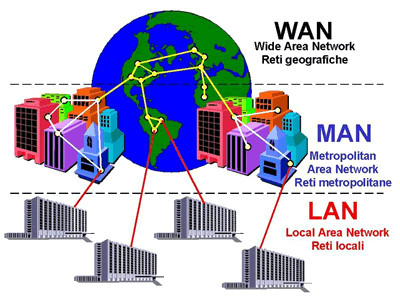
\includegraphics[width=4cm]{partie1/classification.jpg}
\end{wrapfigure}
~

La séparation LAN/WAN va être plus affinée par l'introduction de DAN (Departemental Area Netxork), département au sens de département d'une université, laboratoire, centre, institut; de CAN (Campus Area Network) pour les campus universitaires et de MAN (Metropolitan Area Network), par exemple un réseau de ville. Mais le LAN, MAN et WAN restent les termes les plus utilisés.

~

~

Le choix du critère de distance n'est pas le seul possible. En effet, il est possible d'effectuer les choix suivants:
\begin{itemize}
	\item le débit: Réseau bas débit, moyen débit,haut débit, très haut débit;
	\item le modèle d'architecture: Réseau OSI, X.25, SNA, DNA,DSA\ldots
	\item la gestion: Réseau public, privé
	\item \ldots
\end{itemize}

Des classifications plus fines peuvent être effectuées. Par exemple pour un LAN on distingue:
\begin{itemize}
	\item le réseau autour d'un PABX (Private Automatic Branch eXchange) ou PBX (réseau téléphonique d'une entreprise);
	\item le réseau bureautique (partage d'imprimantes, de logiciels\ldots);
	\item le réseau local industriel (composé de capteurs et d'actionneurs);
	\item le réseau large bande ou intégré ( pour véhiculer le texte, son, image, vidéo);
	\item \ldots
\end{itemize}

